\documentclass[11pt]{article}
\usepackage{amsmath,amsbsy,amssymb,verbatim,fullpage,ifthen,graphicx,bm,amsfonts,amsthm,url}
\usepackage{graphicx}
\usepackage{xcolor}
\newcommand{\mfile}[1]  {{\small \verbatiminput{./#1}}} % Jeff Fessler, input matlab file
\newcommand{\tmop}[1]{\ensuremath{\operatorname{#1}}}
%\newcommand*{\qed}{\hfill\ensuremath{\blacksquare}}%
\newcommand{\R}{\mathbb{R}}
\newcommand{\C}{\mathbb{C}}
\newcommand{\Z}{\mathbb{Z}}
\newcommand{\A}{\mathcal{A}}
\newcommand{\minimize}{\operatorname*{minimize\ }}
\newcommand{\maximize}{\operatorname*{maximize}}
\newcommand{\opdet}[1]{\operatorname{\textbf{det}}\left(#1\right)}
\newcommand{\optr}[1]{\operatorname{\textbf{tr}}\left(#1\right)}
\newcommand{\AnswerDefine}{}
\newcommand{\answer}[2][blue]{\ifdefined\AnswerDefine{\color{#1}\it#2}\fi}
\newcommand{\mtx}[1]{\mathbf{#1}}
\newcommand{\vct}[1]{\mathbf{#1}}
\def \lg       {\langle}
\def \rg       {\rangle}
\def \mA {\mtx{A}}
\def \mB {\mtx{B}}
\def \mD {\mtx{D}}
\def \mE {\mtx{E}}
\def \mF {\mtx{F}}
\def \mG {\mtx{G}}
\def \mI {\mtx{I}}
\def \mJ {\mtx{J}}
\def \mL {\mtx{L}}
\def \mU {\mtx{U}}
\def \mS {\mtx{S}}
\def \mV {\mtx{V}}
\def \mW {\mtx{W}}
\def \mLambda {\mtx{\Lambda}}
\def \mSigma {\mtx{\Sigma}}
\def \mX {\mtx{X}}
\def \mY {\mtx{Y}}
\def \mZ {\mtx{Z}}
\def \zero     {\mathbf{0}}
\def \vzero    {\vct{0}}
\def \vone    {\vct{1}}
\def \va {\vct{a}}
\def \vg {\vct{g}}
\def \vm {\vct{m}}
\def \vu {\vct{u}}
\def \vv {\vct{v}}
\def \vw {\vct{w}}
\def \vx {\vct{x}}
\def \vy {\vct{y}}
\def \vz {\vct{z}}
\def \vphi {\vct{\phi}}
\def \vmu {\vct{\mu}}
\def \R {\mathbb{R}}

%\newcommand{\st}{\operatorname*{\ subject\ to\ }}
\usepackage{algorithm,algpseudocode}
\usepackage{xspace}
% Add a period to the end of an abbreviation unless there's one
% already, then \xspace.
\makeatletter
\DeclareRobustCommand\onedot{\futurelet\@let@token\@onedot}
\def\@onedot{\ifx\@let@token.\else.\null\fi\xspace}

\def\eg{\emph{e.g}\onedot} \def\Eg{\emph{E.g}\onedot}
\def\ie{\emph{i.e}\onedot} \def\Ie{\emph{I.e}\onedot}
\def\cf{\emph{c.f}\onedot} \def\Cf{\emph{C.f}\onedot}
\def\etc{\emph{etc}\onedot} \def\vs{\emph{vs}\onedot}
\def\wrt{w.r.t\onedot} \def\dof{d.o.f\onedot}
\def\etal{\emph{et al}\onedot} \def\st{\emph{s.t}\onedot}
\pagestyle{plain}

\title{{\bf Final Exam, CPSC 8420, Spring 2022}} 
\author{\Large\underline{Last Name, First Name}}% put your name in the LastName, FirstName format
\date{\textbf{\Large\textcolor{red}{Due 05/06/2022, Friday, 11:59PM EST}}} 
%\date{\today}

\begin{document}
\maketitle

\section*{Problem 1 [15 pts]}
Consider the elastic-net optimization problem:
\begin{equation}
\min_{\beta} \|\vy-\mX\beta\|^2+\lambda[\alpha\|\beta\|^2_2+(1-\alpha)\|\beta\|_1].
\end{equation}
\begin{enumerate}
	\item Show the objective can be reformulated into a lasso problem, with a slightly different $\mX, \vy$.
	\item If we fix $\alpha=.5$, please derive the closed solution by making use of alternating minimization that each time we fix the rest by optimizing one single element in $\beta$. You need randomly generate $\mX, \vy$ and initialize  $\beta_0$, and show the objective decreases monotonically with updates.
\end{enumerate}
\answer{You may input your answers here. \LaTeX \ version submission is encouraged.}
\newpage
\section*{Problem 2 [15 pts]}
\begin{itemize}
	\item For PCA, the loading vectors can be directly computed from the $q$ columns of  $\mU$ where  $[\mU,\mS,\mU]=svd(\mX^T\mX)$, please show that any $[\pm\vu_1,\pm\vu_2,\dots,\pm\vu_q]$ will be equivalent to $[\vu_1,\vu_2,\dots,\vu_q]$ in terms of the same variance while satisfying the orthonormality constraint.
	\item We consider the case when original dimensionality of the data is much larger than the number of samples $d\gg m$ ($\mX\in\R^{d\times m}$). What's the complexity of obtaining the optimal solution of PCA via Singular Value Decomposition? Please consider a more efficient solution by considering the relationships of eigenvalues/eigenvectors between $\mX^T\mX$ and $\mX\mX^T$.
\end{itemize}


\newpage
\section*{Problem 3 [10 pts]}
Assume that in a community, there are $10\%$ people suffer from COVID. Assume $80\%$ of the patients come to breathing difficulty while $25\%$ of those free from COVID also have symptoms of shortness of breath. Now please determine that if one has breathing difficulty, what's his/her probability to get COVID? (\textit{hint}: you may consider Naive Bayes)

\newpage
\section*{Problem 4 [20 pts]}
Recall the objective for \text{RatioCut}: $RatioCut(A_1,A_2,...A_k) = \frac{1}{2}\sum\limits_{i=1}^{k}\frac{W(A_i, \overline{A}_i )}{|A_i|}$. If we introduce indicator vector: $h_j \in \{h_1, h_2,..h_k\}, j \in [1,k]$, for any vector $h_j\in R^n$, we define: $h_{ij}= \begin{cases} 0& { v_i \notin A_j}\\ \frac{1}{\sqrt{|A_j|}}& { v_i \in A_j} \end{cases}$, we can prove: $h_i^TLh_i =  \frac{cut(A_i, \overline{A}_i)}{|A_i|}$, and therefore:
\begin{equation}
	RatioCut(A_1,A_2,...A_k) = \sum\limits_{i=1}^{k}h_i^TLh_i = \sum\limits_{i=1}^{k}(H^TLH)_{ii} = tr(H^TLH),
\end{equation}
thus we relax it as an optimization problem:
\begin{equation}
	\underbrace{arg\;min}_H\; tr(H^TLH) \;\; s.t.\;H^TH=I.
\end{equation}
Now let's explore Ncut, with objective:
$NCut(A_1,A_2,...A_k) = \frac{1}{2}\sum\limits_{i=1}^{k}\frac{W(A_i, \overline{A}_i )}{vol(A_i)}$, where $vol(A): = \sum\limits_{i \in A}d_i, d_i: = \sum\limits_{j=1}^{n}w_{ij}$.Similar to Ratiocut, we define: $h_{ij}= \begin{cases} 0& { v_i \notin A_j}\\ \frac{1}{\sqrt{vol(A_j)}}& { v_i \in A_j} \end{cases}$. Now
\begin{enumerate}
	\item Please show that $h_i^TLh_i =\frac{cut(A_i, \overline{A}_i)}{vol(A_i)}$.
	\item Show that $NCut(A_1,A_2,...A_k) = tr(H^TLH)$.
	\item The constraint now is: $H^TDH=I$.
	\item Find the solution to $\underbrace{arg\;min}_H\; tr(H^TLH) \;\; s.t.\;H^TDH=I$.
\end{enumerate}

\newpage
\section*{Problem 5 [10 pts]}
We consider the following optimization problem ($\mY$ is given and generated randomly):
\begin{equation}
	\min_{\mX} \frac{1}{2}\|\mX-\mY\|^2_F + \|\mX\|_*
\end{equation}
where $\mY,\mX\in\R^{100\times100}$ and $\|\cdot\|_*$ denotes the nuclear norm (sum of singular values). Now please use gradient descent method to update $\mX$. ($\frac{\partial \|\mX\|_*}{\partial \mX}=\mU\mV^T$, where $\mU,\mV$ is obtained from reduced SVD, namely $[\mU,\mS,\mV]=svd(\mX,0)$). Plot the objective changes with 1000 iteration.

\newpage
\section*{Problem 6 [20 pts]}
We turn to Logistic Regression:
\begin{equation}
	\min_\beta \sum\limits_{i=1}^{m} ln(1+e^{\lg \beta, \hat{x_i}\rg})-y_{i}\lg \beta, \hat{x_i}\rg, 
\end{equation}
where $\beta=(w;b), \hat{x}=(x;1)$. Assume $m=100, x\in\R^{99}$. Please randomly generate $x, y$ and find the optimal $\beta$ via 1) gradient descent; 2) Newton's method and 3) stochastic gradient descent (SGD) where the batch-size is 1. (need consider choosing appropriate  step-size if necessary). Change $m=1000, x\in\R^{999}$, observe which algorithm will decrease the objective faster in terms of iteration ($X$-axis denotes number of iteration) and CPU time. [You will receive another 5 bonus points if you implement backtracking line search]

\newpage
\section*{Problem 7 [10 pts]}
Please design an (either toy or real-world) experiment  to demonstrate that PCA can be helpful for denoising.
\newpage
\section*{Bonus Problem 8 [10 pts]}
\begin{equation}
	\text{\bf Solve:} \quad \min \|\vx\|_{0} \quad \mbox{s.t.}\quad { \mA \vx = \vy. }
\end{equation}
We have proved that if $\vy = \mA \vx_o$ with
\begin{equation}\label{krank}
	\|\vx_o\|_0 \; \le \; \tfrac{1}{2} \, \mathrm{krank}(\mA).
\end{equation}
Then $\vx_o$ is the unique optimal solution to the  $\ell^0$ minimization problem\index{$\ell^0$ minimization}
\begin{equation}
	\min \|\vx\|_{0} \quad \mbox{s.t.}\quad { \mA \vx = \vy. }
\end{equation}
However, when $\mA$ is of size $5 \times 12$, the following figure illustrates the fraction of success across 100 trials.
\begin{figure}[h!]
	\centering
	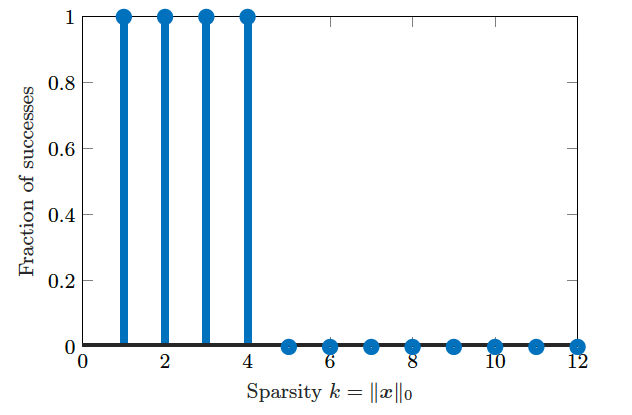
\includegraphics[width=7cm]{simulation-L0.png}
	% \caption{Caption}
	% \label{fig:my_label}
\end{figure}    
Apparently $krank(\mA)\le rank(\mA)\le 5$, therefore, when sparsity $k=1, 2$ satisfying Eq. (\ref{krank}) it has $100\%$ recovery success rate is not surprising. However, the above experiment also shows even $k=3, 4$ which violates Eq. (\ref{krank}), still it can be recovered at $100\%$. Please explain this phenomenon.
%\textbf{Proof:} $
%\mb A \mb \hat{\mb x} = \y \Rightarrow \mb A \left( \hat{\mb x} - \x_o \right) = \mb A \hat{\mb x} - \mb A \x_o = \mb y - \mb y \; = \; \mb 0.$
\end{document}
